%-----------------------------------------------------------------------------%
\chapter{\babTiga}
\thispagestyle{fancy}

%-----------------------------------------------------------------------------%
\section{Tempat dan Waktu Penelitian}
Penelitian tugas akhir ini dilaksanakan di Lab \textit{Strategic Risk Governance} (SRG) Gedung TDMRC USK, Kopelma Darussalam, Kota Banda Aceh. Waktu penelitian ini dilaksanakan selama enam bulan, terhitung dari bulan Agustus hingga Januari 2026.

%-----------------------------------------------------------------------------%
\section{Jadwal Pelaksanaan Penelitian}
Adapun jadwal pelaksanaan penelitian ini dapat dilihat pada distribusi pada Tabel 3.1 dibawah ini.

\begin{table}[h]
\centering
    \renewcommand{\arraystretch}{1.3}
    \renewcommand{\arrayrulewidth}{0.3mm}
    \setlength{\tabcolsep}{4pt}
    \caption{Jadwal Pelaksanaan Penelitian}
    \resizebox{\columnwidth}{!}{
    \begin{tabular}{|c|p{4.5cm}|*{24}{c|}}
        \hline
        \multirow{2}{*}{No} & \multirow{2}{*}{\centering Kegiatan} & \multicolumn{24}{c|}{Bulan Ke -} \\ 
        \cline{3-26}
        & & \multicolumn{4}{c|}{Agustus} & \multicolumn{4}{c|}{September} & \multicolumn{4}{c|}{Oktober} & \multicolumn{4}{c|}{November} & \multicolumn{4}{c|}{Desember} & \multicolumn{4}{c|}{Januari} \\ 
        \hline
        & & 1 & 2 & 3 & 4 & 1 & 2 & 3 & 4 & 1 & 2 & 3 & 4 & 1 & 2 & 3 & 4 & 1 & 2 & 3 & 4 & 1 & 2 & 3 & 4 \\ 
        \hline
        1 & Analisis Kebutuhan & \cellcolor{black} & \cellcolor{black} & \cellcolor{black} &  &  &  &  &  &  &  &  &  &  &  &  &  &  &  &  &  &  &  &  &  \\ \hline
        2 & Studi Literatur &  & \cellcolor{black} & \cellcolor{black} & \cellcolor{black} &  &  &  &  &  &  &  &  &  &  &  &  &  &  &  &  &  &  &  &  \\ \hline
        3 & Preprocessing Data &  &  &  & \cellcolor{black} & \cellcolor{black} & \cellcolor{black} &  &  &  &  &  &  &  &  &  &  &  &  &  &  &  &  &  &  \\ \hline
        4 & Perancangan Sistem &  &  &  &  &  & \cellcolor{black} & \cellcolor{black} & \cellcolor{black} & \cellcolor{black} & \cellcolor{black} & \cellcolor{black} & \cellcolor{black} & \cellcolor{black} & \cellcolor{black} & \cellcolor{black} &  &  &  &  &  &  &  &  &  \\ \hline
        5 & Rancang API &  &  &  &  &  &  &  &  &  &  & \cellcolor{black} & \cellcolor{black} & \cellcolor{black} & \cellcolor{black} & \cellcolor{black} & \cellcolor{black} & \cellcolor{black} & \cellcolor{black} &  &  &  &  &  &  \\ \hline   
        6 & \textit{Smoothing} Dataset &  &  &  &  &  &  &  &  &  &  &  & \cellcolor{black} & \cellcolor{black} & \cellcolor{black} & \cellcolor{black} & \cellcolor{black} & \cellcolor{black} & \cellcolor{black} &  &  &  &  &  &  \\ \hline
        7 & Pengujian Sistem &  &  &  &  &  &  &  &  &  &  &  &  &  &  &  &  &  &  & \cellcolor{black} & \cellcolor{black} & \cellcolor{black} & \cellcolor{black} & \cellcolor{black} & \cellcolor{black} \\ \hline
    \end{tabular}
    }
\end{table}

%-----------------------------------------------------------------------------%

\section{Alat dan Bahan}
Alat dan Bahan yang akan digunakan dalam penelitian ini terdiri dari beberapa perangkat keras (\textit{hardware}) serta perangkat lunak (\textit{software}) yang dijabarkan sebagai berikut: 

\subsection{Perangkat Keras}
Perangkat keras yang digunakan dalam penelitian ini adalah Laptop Lenovo Thinkpad X280 dengan spesifikasi \textit{processor} Intel Core i5-8350U (4 Core 8 Thread) 3.60 GHz, RAM 16GB DDR4, dan memori penyimpanan SSD 1TB.

\subsection{Perangkat Lunak}
Adapun perangkat lunak yang digunakan akan dirincikan sebagai berikut:

\begin{itemize}
    \item OS Arch Linux Kernel 6.6.63-1-lts
    \item Visual Studio Code 1.95.F3
    \item Python 3.12.7
    \item Jupyter v2025.1.0
    \item Flask-API 3.1
    \item Next.js 15 Framework
    \item Google Chrome 132.0.6834.110
    \item MongoDB 8.0.4
    \item Google Earth Engine
    \item PythonAnywhere
    \item Postman API
    \item Cronjob
    \item Draw.io 
\end{itemize}

\section{Prosedur Penelitan}
Prosedur penelitian yang dilakukan terbagi menjadi beberapa tahapan yang dijelaskan pada Gambar \ref{alur_penelitian} di bawah ini. 

\begin{figure}[h]
    \centering
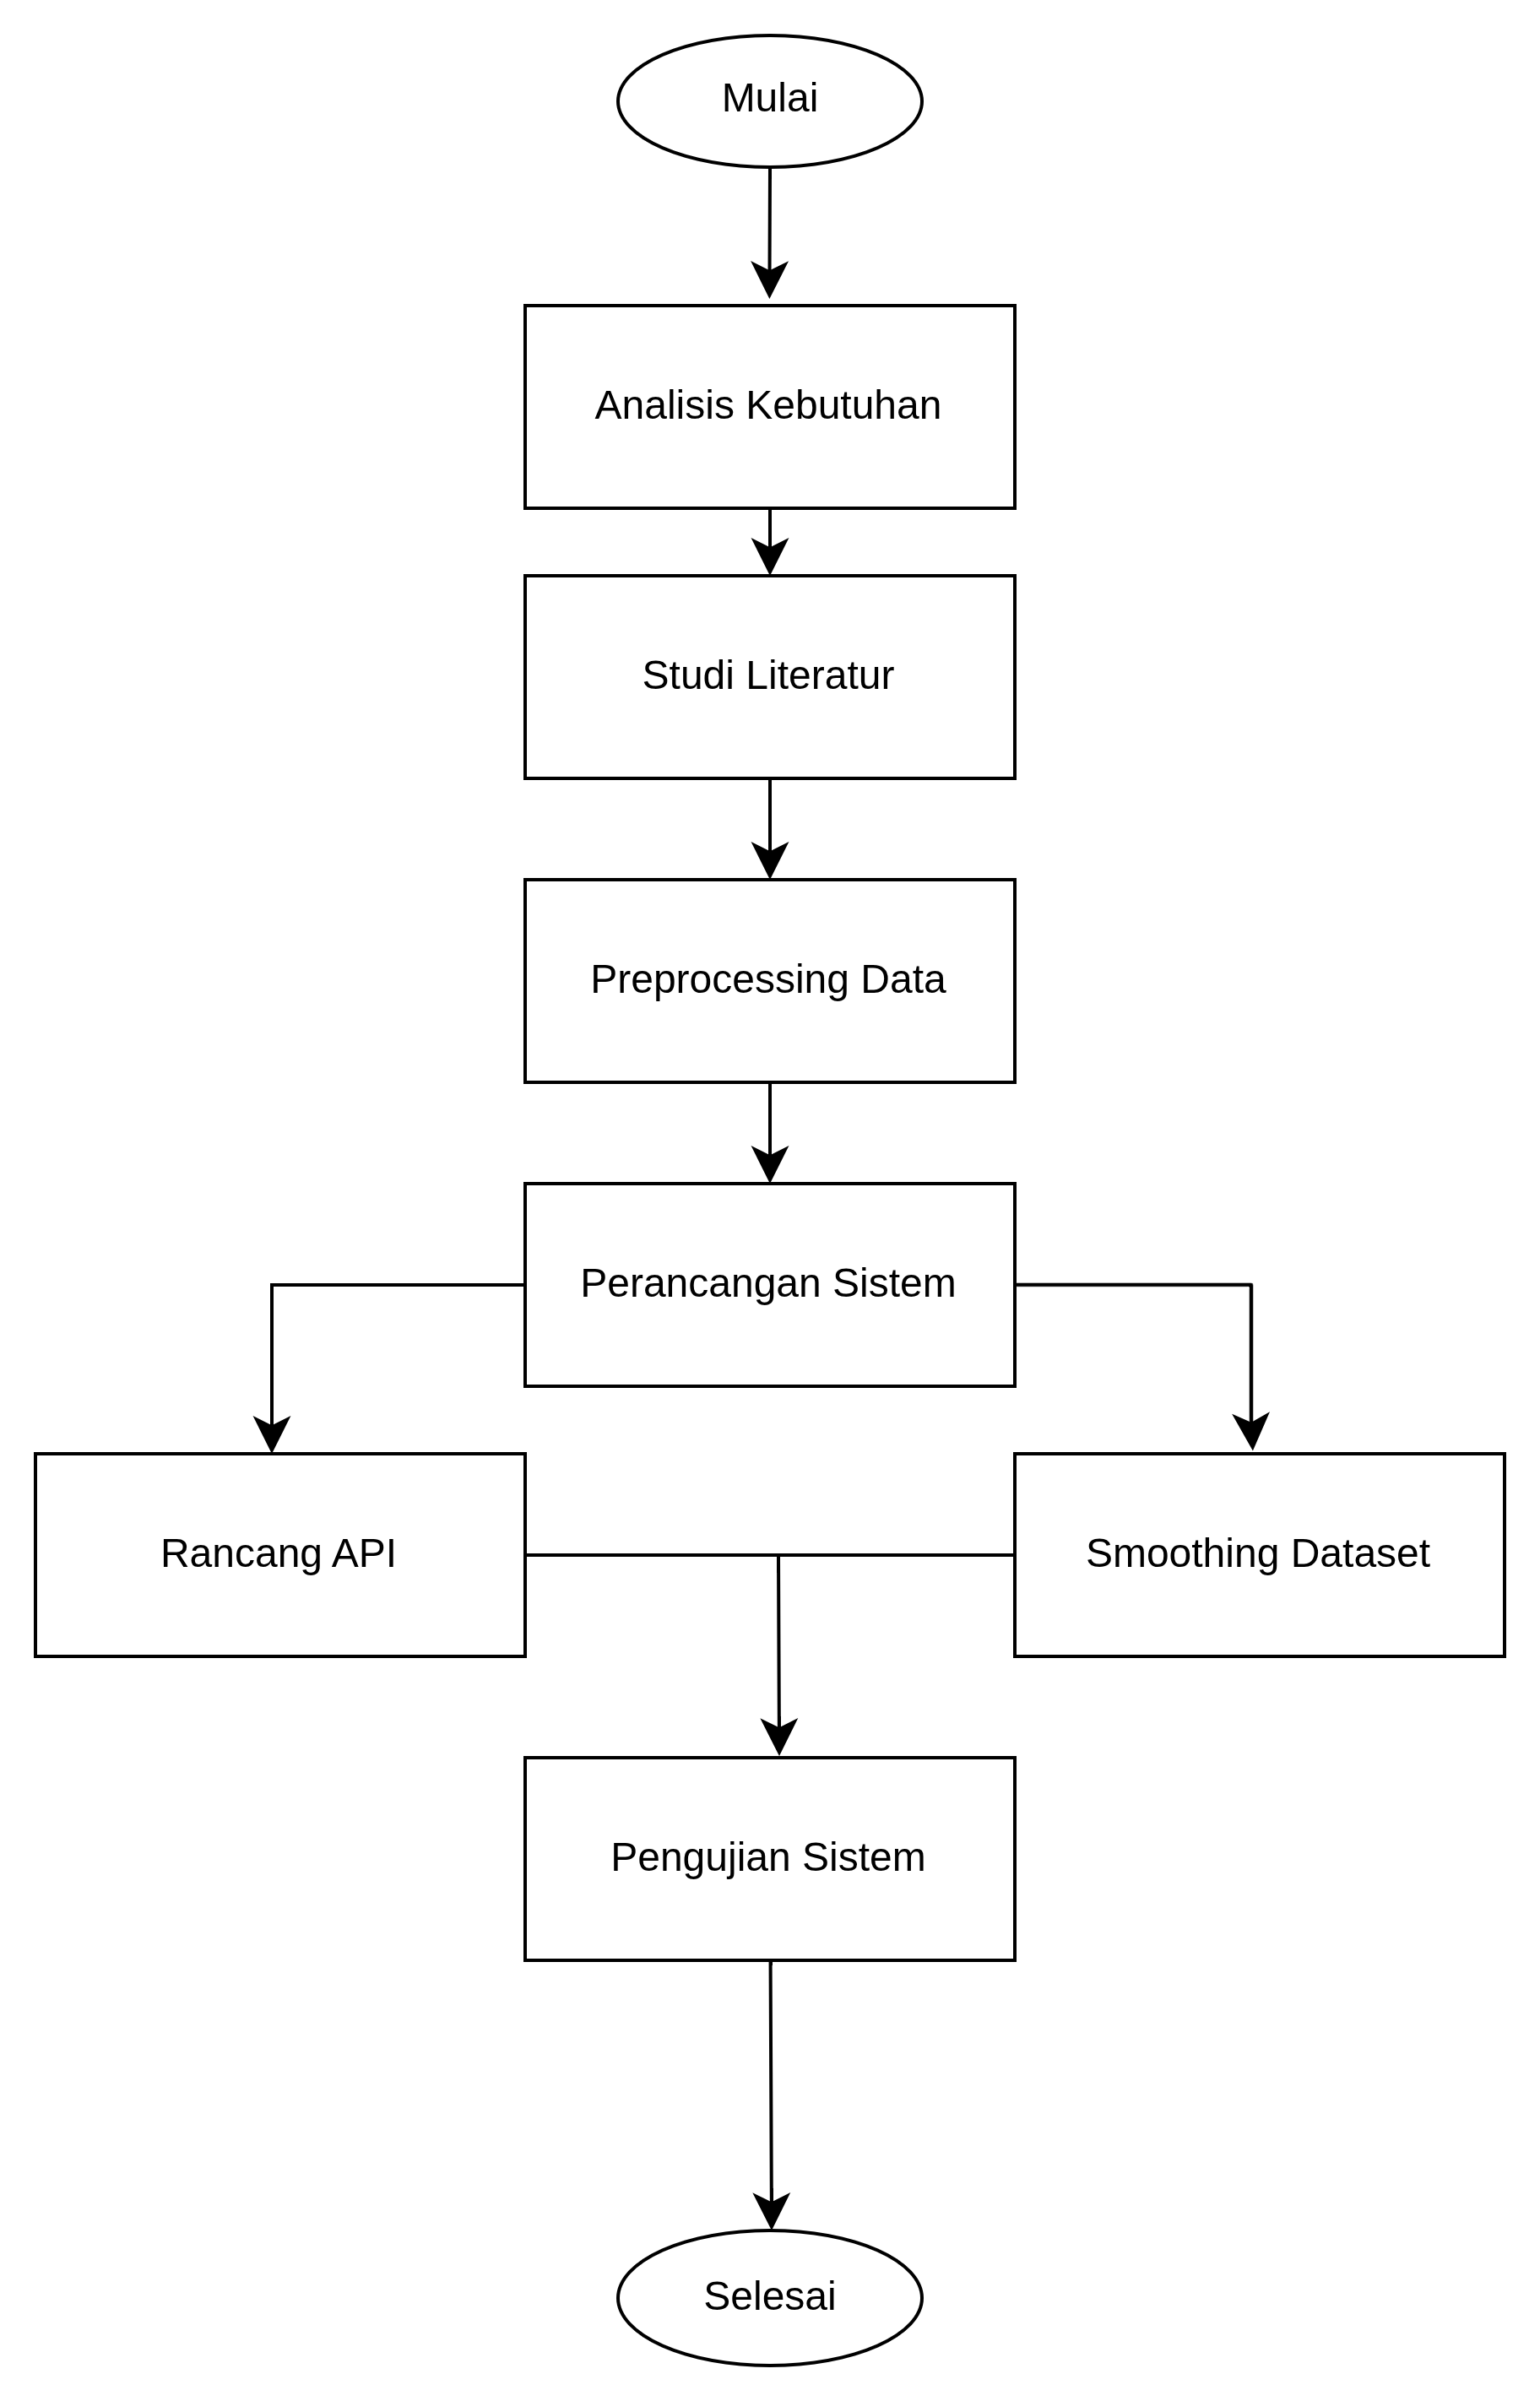
\includegraphics[width=7cm,height=10cm]{assets/pics/bab_iii_alur.png}
    \caption{Diagram Alur Prosedur Penelitian}
    \label{alur_penelitian}
\end{figure}
\subsection{Analisa Kebutuhan}
Langkah awal yang dilakukan dalam penelitian ini adalah analisa kebutuhan, dengan memahami spesifikasi sistem yang akan dikembangkan. Analisis ini mencakup identifikasi kebutuhan pengguna, tujuan penelitian, serta teknologi yang akan digunakan dalam sistem. Pada tahap ini, dilakukan perancangan awal terhadap data iklim yang akan diproses, metode yang digunakan untuk mengolah data tersebut, serta bagaimana data akan disimpan dan disajikan kepada pengguna. Hasil dari tahap ini berupa dokumen spesifikasi kebutuhan sistem yang menjadi dasar dalam tahapan pengembangan berikutnya.

\subsection{Studi Literatur}
Selanjutnya dilakukan studi literatur untuk meneliti teknologi dan metode yang relevan dalam pemrosesan data iklim. Studi ini mencakup penelitian terdahulu mengenai sistem informasi cuaca, metode preprocessing data, serta teknologi yang digunakan dalam pengembangan aplikasi berbasis web. Literatur yang dikaji meliputi jurnal ilmiah, dokumentasi resmi \textit{framework} seperti Next.js untuk \textit{frontend}, Hono untuk \textit{backend}, serta MongoDB untuk integrasi \textit{database} NoSQL. Penelitian ini juga meninjau berbagai pendekatan dalam pemrosesan data iklim, termasuk teknik interpolasi dan normalisasi data yang akan diterapkan dalam sistem.

% \subsection{Mempersiapkan data}
% Data yang digunakan dalam penelitian ini berasal dari sumber eksternal, termasuk dataset cuaca dari BMKG yang berisi parameter seperti suhu, kelembaban, tekanan udara, dan curah hujan. Data ini dapat diperoleh dalam format CSV atau melalui API resmi. Tahapan persiapan data mencakup proses ekstraksi data dari sumber tersebut, penyimpanan dalam database MySQL sementara, serta penyesuaian struktur data agar kompatibel dengan sistem yang akan dikembangkan. Data yang telah dikumpulkan kemudian akan dianalisis untuk mengidentifikasi kemungkinan permasalahan seperti data yang hilang atau duplikat sebelum masuk ke tahap \textit{preprocessing}.

\subsection{\textit{Preprocessing} Data}=
Preprocessing merupakan tahap penting untuk memastikan kualitas data yang digunakan dalam penelitian ini. Pada tahap ini, dilakukan pembersihan data dengan menghapus nilai yang tidak valid atau mengisi data yang hilang dengan teknik interpolasi. Selain itu, data yang masih dalam format mentah akan diubah ke dalam bentuk yang lebih terstruktur sesuai dengan kebutuhan sistem. Normalisasi dan transformasi data juga dilakukan untuk memastikan bahwa informasi dapat digunakan secara optimal dalam analisis maupun penyajian dalam aplikasi. Proses ini dilakukan menggunakan Python dengan \textit{library} seperti pandas, numpy, atau lainnya serta \textit{query} SQL untuk manipulasi data langsung di database.


\subsection{Perancangan Sistem}
Sistem yang dikembangkan dalam penelitian ini dirancang dengan pendekatan \textit{client-server}, di mana \textit{frontend} berbasis Next.js akan berkomunikasi dengan \textit{backend} Hono melalui REST API. Data iklim yang telah diproses akan disimpan dalam database dan diakses melalui API yang telah dirancang. Perancangan sistem ini juga mencakup pembuatan diagram \textit{Entity-Relationship Diagram} (ERD) untuk memodelkan hubungan antar tabel dalam database, serta flowchart untuk menggambarkan alur kerja sistem dari pengambilan data hingga penyajian hasil kepada pengguna. \textit{Data Flow Diagram} (DFD) digunakan untuk menunjukkan bagaimana data mengalir dari satu komponen ke komponen lainnya dalam sistem.


\subsection{Integrasi Database}
Pada tahap ini, sistem menghubungkan \textit{backend} dengan \textit{database} MongoDB untuk menyimpan dan mengelola data iklim yang telah diproses. Struktur \textit{database} dirancang untuk menampung berbagai parameter cuaca dalam tabel yang terstruktur dengan baik, sehingga memudahkan proses pengambilan data untuk analisis lebih lanjut. Integrasi dilakukan menggunakan MongoDB, yang memungkinkan manipulasi database dengan lebih efisien dalam lingkungan Next.js. Dilakukan optimasi \textit{query} agar sistem dapat menangani jumlah data yang besar dengan performa yang tetap optimal.

\subsection{Rancang API}
Untuk memastikan sistem dapat diakses dengan baik oleh frontend dan pihak eksternal, penelitian ini mengembangkan REST API menggunakan framework Hono. API ini menyediakan endpoint untuk melakukan CRUD (\textit{Create, Read, Update, Delete}) terhadap data iklim yang tersimpan dalam \textit{database}. Perancangan API mencakup dokumentasi \textit{endpoint} yang dibuat menggunakan Postman, sehingga memudahkan pengujian dan integrasi dengan sistem lain. Setiap endpoint diuji untuk memastikan keamanan serta efisiensi dalam pengambilan data.

\subsection{Pengujian Sistem}
Setelah sistem selesai dirancang dan dikembangkan, dilakukan pengujian untuk memastikan fungsionalitasnya berjalan sesuai dengan yang diharapkan. Pengujian dilakukan dalam beberapa tahap, termasuk unit testing untuk menguji fungsi-fungsi individu pada API, serta \textit{integration testing} untuk memastikan komunikasi antara \textit{frontend}, \textit{backend}, dan \textit{database} berjalan dengan baik. Load testing dilakukan untuk mengukur performa API dalam menangani permintaan dalam jumlah besar. Pengujian ini dilakukan menggunakan Jest untuk JavaScript/TypeScript, serta JMeter untuk uji beban. Jika ditemukan permasalahan, sistem akan diperbaiki sebelum diimplementasikan secara penuh.
